%\documentclass[aps,amssymb,preprint,a4paper]{revtex4}
\documentclass[aps,amssymb,a4paper,twocolumn]{revtex4}

%\usepackage[latin1]{inputenc}
\usepackage[T1]{fontenc}
\usepackage[english]{babel}
\usepackage{braket}
\usepackage{epsfig}
\usepackage{graphicx}
\usepackage{amsmath,amsfonts,amssymb}
\usepackage{dsfont}
\usepackage{booktabs}
\usepackage{units}
\usepackage{natbib}
\usepackage{xcolor}
\usepackage{multirow}
\usepackage{tikz,pgfplots}
%\usepackage{}
%\usepackage{}
%\usepackage{}

\usetikzlibrary{patterns,shadows,trees,calc}
\usepgfplotslibrary{units}

\pgfplotsset{compat=1.8}

\begin{document}


\newcommand{\wignerj}[6]{\mbox{$\left( \begin{array}{ccc} #1 & #2 & #3 \\ #4 & #5 & #6 \end{array} \right)$}}
\newcommand{\redume}[3]{\mbox{$( #1 || #2 || #3 )$}}

\setlength{\tabcolsep}{12pt}

% Define some colours
\definecolor{diplom1}{rgb}{0.0 0.4 1.0}
\definecolor{diplom2}{rgb}{0.0 0.0 0.6}
\definecolor{diplom3}{RGB}{153,0,0} %unirot

\title{Effect of Spin-Orbit Coupling on Decay Widths of Electronic Decay Processes}

\author{Elke Fasshauer$^{\text{a,b}}$}
\email[]{Email:Elke.Fasshauer@gmail.com}


\affiliation{$^{\text{a}}$Department of Physics and Astronomy,
Aarhus University, Ny Munkegade 120, 8000 Aarhus, Denmark}

\date{\today}

%%%%%%%%%%%%%%%%%%%%%%%%%%%%%%%%%%%%%%%%%%%%%%%%%%%%%%%%
%                  Abstract                            %
%%%%%%%%%%%%%%%%%%%%%%%%%%%%%%%%%%%%%%%%%%%%%%%%%%%%%%%%
\begin{abstract}
Auger-Auger-Meitner processes are electronic decay processes of energetically low-lying
vacancies. In these processes, the vacancy is filled by an electron of
an energetically higher lying orbital, while another electron is simulataneously
emitted to the continuum.
In low-lying orbitals relativistic effects can not even be neglected for light
elements. At the same time lifetime calculations are computationally expensive.
In this context, we investigate which effect spin-orbit coupling has on
Auger-Meitner
decay widths and aim for a rule of thumb for the relative decay widths of
initial states split by spin-orbit coupling.
We base this rule of thumb on Auger-Auger-Meitner decay widths
of Sr$4p^{-1}$ and Ra$6p^{-1}$
obtained by relativistic FanoADC-Stieltjes calculations.
\end{abstract}


\maketitle


%%%%%%%%%%%%%%%%%%%%%%%%%%%%%%%%%
% Introduction
%%%%%%%%%%%%%%%%%%%%%%%%%%%%%%%%%
\section{Introduction}


%%%%%%%%%%%%%%%%%%%%%%%%%%%%%%%%%%%%%%%%%%%%%%%%%%%%
%%%%%%%%%  Theory
%%%%%%%%%%%%%%%%%%%%%%%%%%%%%%%%%%%%%%%%%%%%%%%%%%%%
\section{Theory}
\label{section:theory}

Following Wentzel \cite{Wentzel27} and later Feshbach \cite{Feshbach58,Feshbach62}
and Fano \cite{Fano61}
the decay width of a decay process initiated by a
primary ionization is given by 

\begin{equation} \label{equation:Fano_golden}
  \Gamma = \sum_\beta 2\pi
           \left| \braket{\Phi|\hat{V}|\chi_{\beta,\varepsilon}} \right|^2 .
\end{equation}

Here, $\ket{\Phi}$ and $\ket{\chi_{\beta,\varepsilon}}$ denote the initial and
final state, respectively. $\hat{V}$ is the interaction operator of the
initial and final states, which in Feshbach's definitions is known as $H_{PQ}$.
The index $\beta$ counts the different
decay channels and $\varepsilon$ denotes the energy of the final state.
Eq. (\ref{equation:Fano_golden}) thereby connects the metastable initial
and the continuum final states. They are constructed by partitioning the
Hamiltonian into two subspaces. The initial (final) state is then an
eigenfunction of this initial (final) state sub-space Hamiltonian.
However, finding proper solutions to both the initial and the final
states on an equal footing is a non-trivial task, because they adhere to
different boundary conditions. Since the final state depends on the energy
of the emitted electron, any approach needs to either determine the continuum
state or to mimic the final state using $\mathcal{L}^2$-functions.
While the continuum functions are normalized with respect to their energy

\begin{equation}
 \braket{\chi_\varepsilon| \chi_{\varepsilon'}} = \delta(\varepsilon-\varepsilon')
\end{equation}

the $\mathcal{L}^2$ approach is based on a discrete set of final states
$\ket{\tilde{\chi}_{\tilde{E}}}$
which adhere to different boundary
conditions and are normalized with respect to space (see e.g. \cite{Craigie14}):
\begin{equation}
 \braket{ \tilde{\chi}_{\tilde{E}_i} | \tilde{\chi}_{\tilde{E}_j} } = \delta_{ij}.
\end{equation}

Because of this different normalization the decay widths are not amenable to
a direct calculation. As first proposed by Hazi \cite{hazi1978}, for
autoionization processes such difficulties
can be solved by using the
Stieltjes-Chebyshev moment theory also called Stieltjes imaging
\cite{Langhoff76,Corcoran77,MuellerPlathe90}.
It relies on the observation that the moments of the projected final
state Hamiltonian $H_f$

\begin{equation}
 \mu_k = \braket{ \Phi | \hat{V} H^k_f \hat{V} | \Phi }
\end{equation}

calculated from the determined
discrete pseudo-spectrum are good approximations to the moments determined
from the real continuum states.
This can be shown by inserting the resolution of identity for
the continuum states

\begin{equation}
 \mu_k = \sum_i \varepsilon_i^k
         \left| \braket{ \Phi | \hat{V} | \chi_{i,\varepsilon} } \right| ^2
       + \int\limits_{E_{thr}}^{\infty} \varepsilon^k
         \left| \braket{\Phi|\hat{V}|\chi_{\varepsilon}} \right|^2 \mathrm{d}\varepsilon  .
\end{equation}

Since the non-zero contribution to the coupling matrix elements in the
Feshbach-Fano approach stem only
from an interaction region of finite size, where the $\mathcal{L}^2$ final
state functions are nonvanishing, we may replace the expansion
$\sum\limits_i \ket{\chi_{i,\varepsilon}} \bra{\chi_{i,\varepsilon}}
 + \int \mathrm{d}\varepsilon \ket{\chi_\varepsilon} \bra{\chi_\varepsilon}$
by its $\mathcal{L}^2$ approximation
$\sum\limits_j \ket{\tilde{\chi}_{\tilde{E}_j}} \bra{\tilde{\chi}_{\tilde{E}_j}}$
(see \cite{Reinhardt79})

\begin{equation}
 \label{eq:moment_discrete}
 \mu_k \approx \sum\limits_j \tilde{E}_j ^k
         \left| \braket{\Phi|\hat{V}|\tilde{\chi}_{\tilde{E}_j}}  \right|^2 .
\end{equation}

Then the decay width can be determined through a series of
consecutive approximations to the moments of increasing order $k$.

To achieve this kind of description, we choose the non-relativistic
FanoADC-Stieltjes approach.
Here, the ADC is used for the description of the
initial and final states and the resulting discrete pseudo-spectrum
is then subject to a Stieltjes imaging procedure.
An exhaustive description of the method can be found in \cite{Fasshauer15,Fasshauer_thesis}.


%%%%%%%%%%%%%%%%%%%%%%%%%%%%%%%%%%%%%%%%%%%%%%%%%%%%
%%%%%%%%%  Computational Details
%%%%%%%%%%%%%%%%%%%%%%%%%%%%%%%%%%%%%%%%%%%%%%%%%%%%
\section{Computational Details}
\label{section:computational}
The Auger-Meitner
decay widths were calculated with the relativistic FanoADC-Stieltjes
method
implemented in the relativistic quantum chemical program DIRAC \cite{DIRAC17}.
We included up to third order contributions of perturbation theory and additional
constant diagrams.
For each element four-component calculations based on the
Dirac-Coulomb (DC) Hamiltonian
and scalarrelativistic spinfree calculations were
performed for both the $(n-1)p_{1/2}$ and $(n-1)p_{3/2}$ initial states.
Dyall's cv4z basis sets \cite{Dyall4s-7s09} were augmented with additional diffuse
5s5p5d3f
basis functions following the Kaufmann-Baumeister-Jungen approach
\cite{Kaufmann89}.
The resulting moments were checked for numerical instabilities.
Only those moments, without numerical instabilities entered the interpolation
scheme for the determination of the decay widths.\\
The radial orbital densities of the ions were calculated using GRASP
\cite{Dyall89,Parpia96}.


%%%%%%%%%%%%%%%%%%%%%%%%%%%%%%%%%%%%%%%%%%%%%%%%%%%%
%%%%%%%%%  Results and discussion
%%%%%%%%%%%%%%%%%%%%%%%%%%%%%%%%%%%%%%%%%%%%%%%%%%%%
\section{Results}
\label{section:results}

\begin{figure}[h]
 \centering
 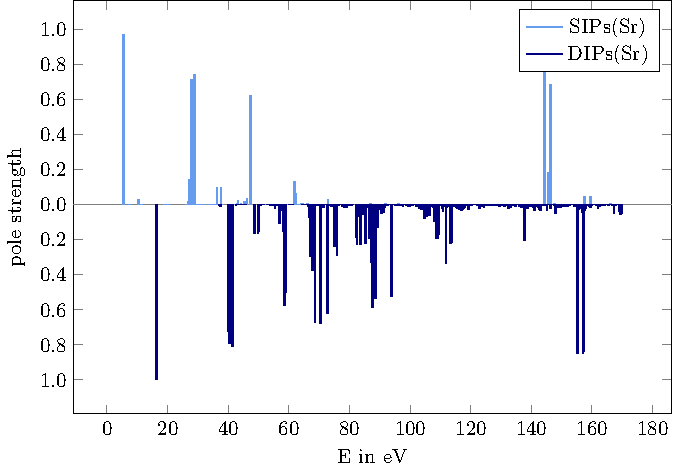
\includegraphics[width=0.9\columnwidth]{pics/Sr_rel_sdip.pdf}
 \caption{Comparison of the single (SIP) and double (DIP) ionization spectra
          of the strontium obtained by a DC-ADC calculation.}
 \label{fig:sdip}
\end{figure}

\begin{table}[h]
 \centering
 \caption{}
 \begin{tabular}{lrrr}
  \toprule
   initial state    & energy $[\unit{eV}]$ & ps & $\Gamma [\unit{meV}]$\\
  \midrule
   Sr spinfree      & 28.599 & 0.78 &   0.56\\  
   Sr$4p_{1/2,1/2}$ & 29.402 & 0.80 &   0.10\\
   Sr$4p_{3/2,1/2}$ & 28.277 & 0.76 &   1.23\\
   Sr$4p_{3/2,3/2}$ & 28.277 & 0.76 &   1.17\\
%  \midrule
%   Ba$5p_{1/2,1/2}$ & 25.108 & 0.80 & unreliable\\
%   Ba$5p_{3/2,1/2}$ & 23.106 & 0.76 &   55.9\\
%   Ba$5p_{3/2,3/2}$ & 23.106 & 0.76 &   63.1\\
  \midrule
   Ra spinfree      & 21.836 & 0.49 &  28.56 \\  
   Ra$6p_{1/2,1/2}$ & 25.494 & 0.78 &   0.26\\
   Ra$6p_{3/2,1/2}$ & 19.267 & 0.50 &  93.16 \\
   Ra$6p_{3/2,3/2}$ & 19.267 & 0.50 &  98.86\\
  \bottomrule
 \end{tabular}
 \label{tab:widths}
\end{table}



\begin{align*}
 (n-1)p^{-1} \,ns^2         \rightarrow & (n-1)p^6 + e^- \\
 (n-1)p^{-1} \,(n-1)d \, ns \rightarrow & (n-1)p^6 + e^- \\
 (n-1)p^{-1} \,(n-1)d^2     \rightarrow & (n-1)p^6 + e^- \\
\end{align*}


\begin{figure}[h]
 \centering
 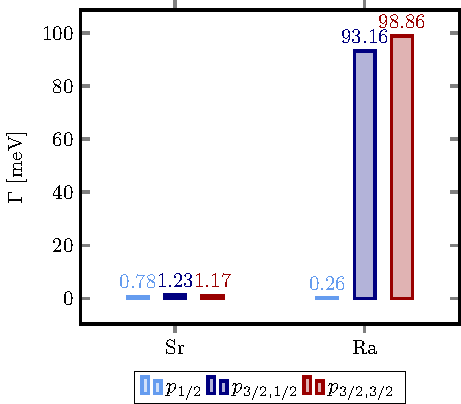
\includegraphics[width=\columnwidth]{pics/sr_ba_ra.pdf}
\end{figure}

\begin{figure}[h]
 \centering
 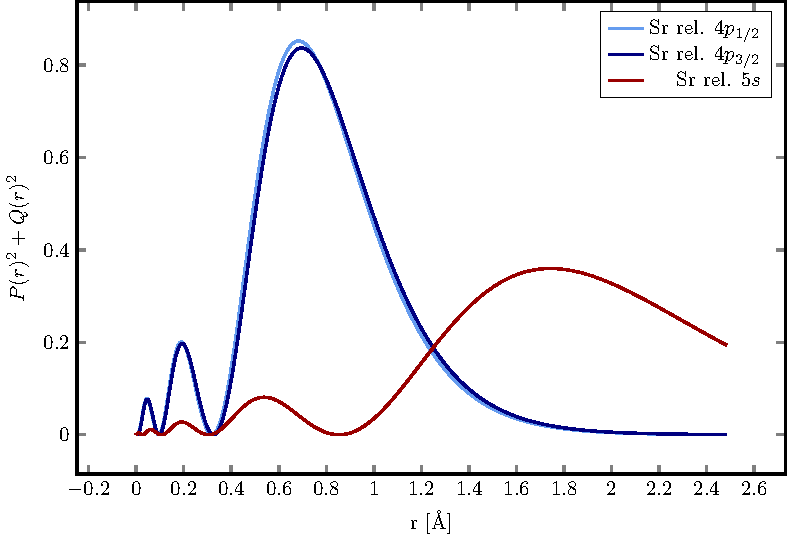
\includegraphics[width=\columnwidth]{pics/sr_ion_R.pdf}\\
 %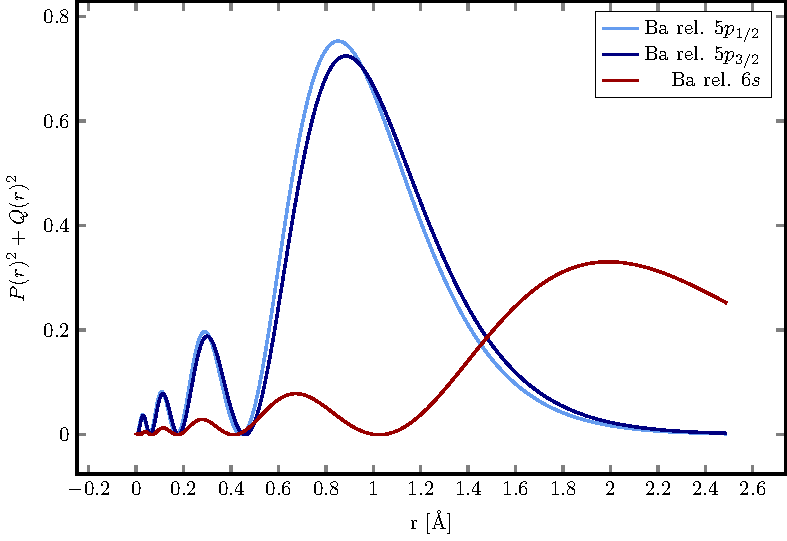
\includegraphics[width=\columnwidth]{pics/ba_ion_R.pdf}\\
 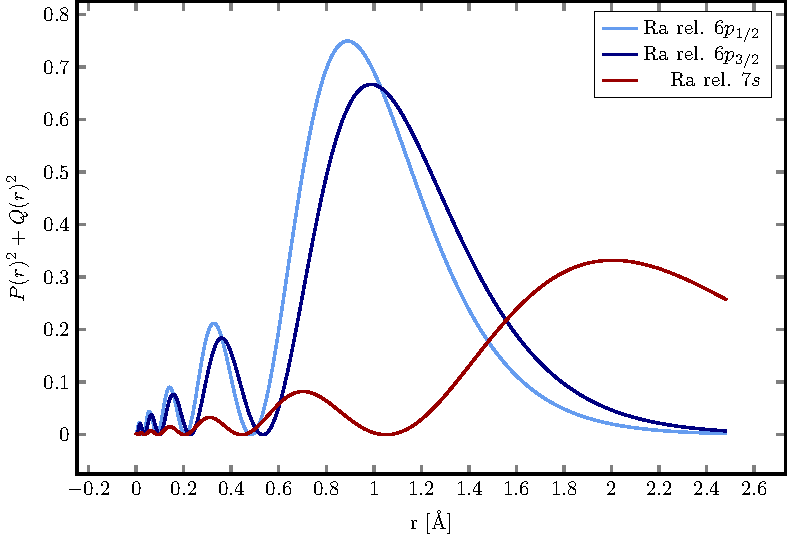
\includegraphics[width=\columnwidth]{pics/ra_ion_R.pdf}\\
 \caption{Radial densities of the orbitals of the $(n-1)p^5s^2$ ions
          involved in the Auger decay.
          The expectation value of the electrons position of the $(n-1)p_{1/2}$
          orbital is lower than of the respective $(n-1)p_{3/2}$
          orbitals. The $ns$ orbitals of the ions experience a stronger
          contraction the those of the atom (not shown here).}
 \label{fig:radial}
\end{figure}




\begin{figure}[h]
 \centering
 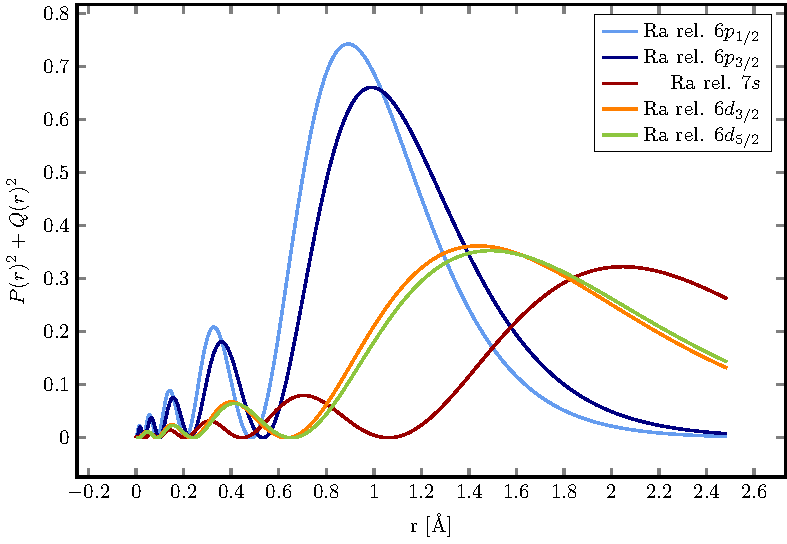
\includegraphics[width=\columnwidth]{pics/ra_6d_R.pdf}
 \caption{Radial densities of the radium orbitals of the ionic $6p^5 6d 7s$
          configuration involved in the Auger decay. The overlap of the radial
          densities of the $6p$ orbitals with the radial densities of the $6d$ orbitals
          is more pronounced than with the radial density of the $7s$ orbital.}
 \label{fig:radial}
\end{figure}


%%%%%%%%%%%%%%%%%%%%%%%%%%%%%%%%%%%%%%%%%%%%%%%%%%%%
%%%%%%%%%  Conclusions
%%%%%%%%%%%%%%%%%%%%%%%%%%%%%%%%%%%%%%%%%%%%%%%%%%%%
\section{Conclusions}
\label{section:conclusions}

\section{Acknowledgements}
The author would like to thank the audience of the REHE 2017 conference for
raising the main question addresed in this article
and acknowledges funding from the Villum foundation.


\clearpage

%\bibliographystyle{apsrev4-1}
%\bibliography{theolit}

\end{document}
